\documentclass[12pt]{article}
\usepackage[T1]{fontenc}
\usepackage[utf8]{inputenc}
\usepackage{amsmath}
\usepackage{lmodern}\title{LTE-M}
\usepackage{mathtools}
\usepackage{graphicx}
\newcommand\tab[1][1cm]{\hspace*{#1}}
\DeclarePairedDelimiter\floor{\lfloor}{\rfloor}
\author{Artur Ziemba  \\
	Zachodniopomorski Uniwersytet Technologiczny w Szczecinie}
\date{\today} 

\begin{document}

\maketitle
\pagebreak

\tableofcontents %spis tresci

\pagebreak
\section{What is M2M?}
\subsection{Brief}
M2M is defined as data communication among devices without the need for human interaction. This may be data communication between devices and a server, or device-to-device either directly or over a network.\\
Examples of M2M services include security, tracking, payment, smart grid and remote maintenance/monitoring. 

\subsection{Technical information}
LTE-M, which is an abbreviated version of LTE-MTC (or “machine-type communications”), is a part of 3GPP’s release, and it is still under consideration.\\
The LTE channel is made up of resource blocks of about 230 kHz of spectrum, and LTE-M is part of the 1.4 MHz block, comprised of six resource blocks.\\
The advantage of LTE-MTC for M2M communications is that it works within the normal construct of LTE networks. Other words, a cellular carrier like AT\&T  only has to upload new baseband software onto its base stations to turn on LTE-M and won’t have to spend any money on new antennas. It’s also five times simpler than a category 4 receiver—like that found in user equipment like a cell phone—because it needs only to understand and digitize 1.4 MHz of the channel instead of 20 MHz
LTE-M has a little higher data rate than NB-LTE-M and NB-IoT, but it is able to transmit fairly large chunks of data. Thus, it can be used for applications such as tracking objects, wearables, energy management, utility metering, and city infrastructure. 

\subsection{Architecture}
\begin{center}
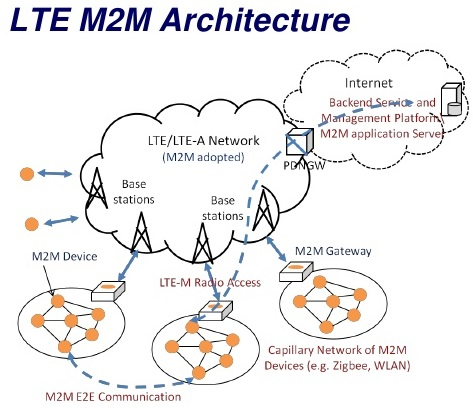
\includegraphics[width=16cm,height=15cm]{image.jpg}
\pagebreak
\end{center}

\subsection{Why Cat-M}
The Internet of Things, IoT and machine to machine, M2M communications are growing rapidly.\\
LTE, the Long Term Evolution cellular system is well placed to carry a lot of the traffic for machine to machine communications.
The issue is that LTE is a complex system capable of carrying high data rates.\\
Associated with it are new categories being launched known as LTE Cat 1.4MHz and LTE Cat 200kHz.

\pagebreak
\section{Requirements}
\begin{enumerate}
\item Wide spectrum of devices   
\item Low devices cost
\item Long battery life 
\item Enhanced coverage   
\item Large volumes - low data rates
\item Low deployment cost
\end{enumerate}
 
\begin{description}
\subsection{Wide spectrum of devices}
\item[\label{Wide spectrum of devices}]{
\tab Any LTE machine to machine system must be able to support a wide variety of different types of devices. These may range from smart meters to vending machines and security and medical devices. These different devices have many differing requirements, so any LTE-M system needs to be able to be flexible}

\subsection{Low devices cost}
 \item[\label{Low devices cost}]{
 \tab Most M2M devices need to be small and fit into equipment that is very cost sensitive. With many low cost M2M systems already available, LTE-M needs to provide the benefits of a cellular system, but at low cost
\begin{enumerate}
\item Reduced UE receive bandwidth to 1.4 MHz allows for substantial complexity reduction
\item The UE will still be able to operate in all existing LTE system bandwidths up to 20 MHz
\item A lower UE power class will allow integration of power amplifier in single chip solution
\end{enumerate}
}
\subsection{Long battery life}
 \item[\label{Long battery life}]{
\tab Many M2M devices will need to be left unattended for long periods of time in areas where there may be no power supply. Maintaining batteries is a costly business and therefore any devices should be able to have a time between battery changes of up to ten years. This means that the LTE-M system must be capable of draining very little battery power. \\
For improved battery life 3GPP introduces a UE power saving mode. UE performs periodic tracking area update (TAU) after which it stays reachable for paging during a configurable Active timer before it goes to sleep (not reachable).\\
More than 10 years battery lifetime with 2 AA batteries can be achieved for delay - tolerant traffic if the TAU cycle is 10 minutes\\\\
\begin{tabular}{|l|c|c|c|c|c|c|c|}
\hline
trans / cycle & 2.56 s &10.24 s & 1 min & 10 min & 1 h & 2 h & 1 day \\
\hline 
15 min & 3.7 & 4.5 & 4.9 & 4.9 & 4.9 & 4.9 & 4.9 \\
\hline 
1 h & 8.1 & 13.8 & 17.0 & 17.8 & 17.9 & 17.9 & 17.9 \\
\hline 
1 day & 13.2 & 39.1 & 84.9 & 108.0 & 110.8 & 111.1 & 111.3 \\
\hline 
1 week & 13.5 & 42.0 & 99.4 & 132.1 & 136.2 & 136.6 & 137.0 \\
\hline 
1 month & 13.6 & 42.3 & 101.6 & 135.9 & 140.2 & 140.7 & 141.1 \\
\hline 
1 year & 13.6 & 42.5 & 102.3 & 137.1 & 141.4 & 141.9 & 142.3 \\
\hline 
\end{tabular} 
}

\subsection{Enhanced coverage}
 \item[\label{Enhanced coverage}]{
\tab LTE-M applications will need to operate within a variety of locations - not just
where reception is good. They will need to operate within buildings, often in
positions where there is little access and where reception may be poor.
Accordingly LTE-M must be able to operate under all conditions.
} 

\pagebreak
\subsection{Large volumes - low data rates}
 \item[\label{Large volumes - low data rates}]{
\tab As it is anticipated that volumes of remote devices will be enormous, the
LTE-M must be structured so that the networks are be able to
accommodate vast numbers of connected devices that may only require
small amounts of data to be carried, often in short peaks but with low data
rates. 
}

\subsection{Low deployment cost}
 \item[\label{Low deployment cost}]{
 \tab LTE-M operates on a 1.4 MHz carrier or 6 PRB. The IoT device will always listen to the center 6
PRB for control information like any normal device. When the device is scheduled for IoT traffic, it
will be allocated a number of PRBs (up to 6) at any consecutive location within the spectrum of
operation. This means that the device will be allocated a 1.4 MHz carrier within a, for example, 20
MHz carrier.\\
The dedicated control and data is multiplexed in the frequency domain ignoring the legacy control
information. This enables LTE IoT devices to be scheduled within any legacy LTE system and
share the carrier capacity, antenna, radio and hardware at the site. 

} 
\end{description}

\pagebreak
\section{CatM Frequency Hopping}
\subsection{Narrowbands}
Narrowband is a contiguous band of 72 subcarriers (6 PRBs).
NB is maximum bandwidth supported by CatM UE both in DL and UL.
\subsection{Narrowbands per bandwidth}
\begin{center}
\begin{tabular}{|c|c|c|c|c|c|c|}
\hline
BW & 1.4 MHz & 3 MHz & 5 MHz & 10 MHz & 15 MHz & 20 MHz  \\
\hline 
subcarriers & 72 & 180 & 300 & 600 & 900 & 1200  \\
\hline 
PRB & 6 & 15 & 25 & 50 & 75 & 100 \\ 
\hline 
narrowbands & 1 & 2 & 4 & 8 & 12 & 16 \\
\hline 
\end{tabular} 
\end{center}

\subsection{Frequency hopping}
Frequency Hopping is the technique of cyclic moving the transmission in frequency through the available bandwidth, according to the predefined pattern. The reason of using FH is the diversification of used spectrum in order to increase transmission robustness.

\subsection{Technical information}
Subframe (not slot) based
Defined in terms of PRBs, similarly but not identically as in legacy.
UE has to retune frequency between hops, PRBs are located in different NBs.
Defined in terms of only Narrowband changes between hops.
Formulas prevent allocation in center NBs.
The hopping pattern depends on BW (no hops for 1.4 MHz, 2 hops for 3-10 MHz, 4 hops for 15-20 MHz) and Cell ID.



\subsection{Frequency hoping pattern}
\begin{align*}
\begin{multlined} \\
N_{nb}=s_j  \\
j=(N_{cell}\bmod N_{s nb}+i*\floor*{N_{snb}/m})\bmod N_{snb} \\
i=0,1,\cdots,m-1 \\
m = \left\{
\begin{array}{ll}
1 & \mbox{if } N_{DLrb} < 12 \\
2 & \mbox{if } 12 \leq N_{DLrb} \leq 50 \\
4 & \mbox{if } 50 < N_{DLrb} \\
\end{array}\right.  \\ 
\end{multlined}
\end{align*}

\paragraph{where:\\}
$s_j$ - set of narrowbands \\
$N_{cell}$ - physical cell id \\
$N_{snb}$ - number of NBs in the set \\
$N_{DL}$ - number of RBs \\
$m$ - number of hops \\

\pagebreak
\section{Conclusions}\label{conclusions}
In 2020, the average mobile subscriber will use several Gbytes of mobile broadband data per day. By contrast, a connected ‘thing’ may use hundreds of kbytes per day on average. The IoT traffic will in this example only consume about 0.01 percent of the mobile broadband data. Furthermore, most of the IoT traffic will not follow the same peak data consumption as mobile broadband and most IoT traffic can be scheduled overnight. Therefore, deploying LTE-M and NB-IoT is as simple as a software upgrade to enable a full IoT network with significantly better coverage than the legacy LTE network.\\
IoT changes the requirements for connectivity significantly, mainly with regards to long battery life, low
device costs, low deployment costs, extended coverage and support for a massive number of devices.
Based on these requirements, several different non-cellular LPWA connectivity solutions are emerging and
are competing for IoT business and the overall connectivity market. 

\pagebreak
\begin{thebibliography}{9}
\bibitem{Cox} 
Christopher Cox
\textit{AN INTRODUCTION
TO LTE}.
LTE, LTE-ADVANCED, SAE
AND 4G MOBILE COMMUNICATIONS 2012.

\bibitem http://www.radio-electronics.com/info/cellulartelecomms/lte-long-term-evolution/lte-m-m2m-machine-to-machine.php
\end{thebibliography}

\end{document}

